The system described in Section \ref{sys} is modeled and simulated in MATLAB\textsuperscript{\textregistered} Simulink\textsuperscript{\textregistered} using the Simscape Power Systems\textsuperscript{TM} toolbox in phasor domain for the Offline simulation. The A* based ESM is run using the described data, and the results are fed in as an open loop control to a Simulink model for phasor simulation. In the test cases, the energy management problem is formulated according to the formulation discussed in Section \ref{formulation}. The  SOC of the ESS is discretized in steps of 2\%, and the SOC is limited between  94\%  and  10\%. The time step and the control horizon chosen is 15 minutes. The ES is allowed to charge or discharge a maximum of 8\% of its total capacity during one time-step. The 8\% limitation is set based on the power specifications discussed in table \ref{tab:es}. The A* search runs every 15 minutes considering a 24 hours (96 time-steps) prediction horizon. The performance of the A* based ESM is compared against two sample base test cases. The base test cases are the following:

\begin{enumerate}
\item \textbf{Case 1:} Charging the ES from 2 AM to 5 AM, Discharging the ES from 7 PM to 11 PM

\item \textbf{Case 2:} Charging from the ES 11 AM to 2 PM, Discharging the ES from 7 PM to 11 PM
\end{enumerate}

All the test cases are run under two different scenarios. Scenario I considers net metering scheme and  Scenarios II considers different prices for buying and selling energy.

\subsection{Scenario I: Net Metering} \label{netmeter}
In this scenario, the A* based EMS is compared against the two base test cases considering net metering. The NYISO RTP scheme shown in Fig. \ref{fig:RTP_PROFILE_8} is used for this comparison. The price of the energy storage is chosen as 12.6 \cent/kWh. This price is calculated based on the specifications of the Tesla Powerpack \cite{tesla_powerpack_2018}. \textcolor{blue}{Besides the tow base test cases genetic algorithm (GA) and sequential quadratic programming based (SQP) approaches has also been used to create comparison cases for this scenario.
The total costs of these cases are shown in Table \ref{tab:Cost1}.}

\textcolor{blue}{
\textbf{GA case:} In this case GA was used to find the minimum cost of (\ref{eq:C_actual}) in every time step. The GA used a population size of 150. Increasing population size over this number did not show significant improvement and increased computation time significantly. The genetic algorithm solver available with MATLAB\textsuperscript{\textregistered} \cite{GA} was used to find the minimum cost of  (\ref{eq:C_actual}) while maintaining the ES charging and discharging constraints mentioned before (ES can charge and discharge a maximum of 8\% of total capacity and SOC is kept between 10\% to 94\%).
}

\textcolor{blue}{
\textbf{SQP case:} In this case SQP was used to find the minimum cost of (\ref{eq:C_actual}) in every time step. The SQP solver available with the fmincon function in  MATLAB\textsuperscript{\textregistered} \cite{SQP} was used to obtain the minimum cost of (\ref{eq:C_actual}) at every time step. The constraints for the SQP approach are the same as the GA approach.}

Fig. \ref{fig:SBMPO_COMP_1_day} shows a zoomed view of the first day of the 7-day simulation for the A* based EMS. The solid black line in the figure represents the SOC of the energy storage, and the dotted red line represents the RTP. The dashed blue line represents the apparent demand. The left vertical axis of the graph represents the RTP of energy and the SOC of the ES. The right vertical axis represents the kWh apparent demand (actual demand - PV generation) of the system. A negative apparent demand represents excess energy from the local generation after fulfilling the local demand. The horizontal axis represents time in hours. The arrows with the numbers are showing specific points of the figure that are explained next, based on the behavior of the EMS. As observed in Fig. \ref{fig:SBMPO_COMP_1_day}, there are two peaks in price at points 1 and 3 throughout the 24 hours window of operation. The ESM accurately anticipates the price peak in point 1 and charges the energy storage using the grid just before the peak occurs, and discharges during the price peak at point 1. It can be seen that during the peak, the apparent demand was positive and the cheapest available price for grid energy was available just before the peak. The algorithm also anticipates the next price peak at point 3 based on forecasted data and prepares the ES to discharge at that price peak by charging at the lowest RTP period at point 2. Although, there is excess generation available from the PV in between point 2 and point 3 the opportunity cost of using the PV to charge the ES will be equal to the RTP due to net metering. So, in this case, the algorithm behaves as expected and uses the lowest possible RTP period to charge the ES and discharges during the price period when there is a high enough price peak to justify the use of the energy storage.

\begin{figure}[!ht]
    \centering
    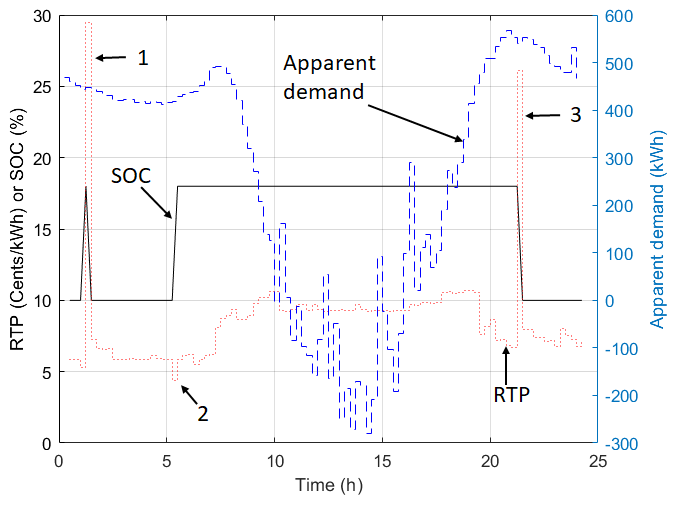
\includegraphics[width = 0.8\linewidth]{figs/SBMPO_COMP_1_day.png}
    \caption{First day EMS response for net metering comparison case}
    \label{fig:SBMPO_COMP_1_day}
\end{figure}

Fig. \ref{fig:SBMPO_COMP_10_12} shows the response of the A*-based EMS in a seven-day run used in the same microgrid system.  It can be seen from the figure that the A*-based ESM is following the same behavior displayed in Fig. \ref{fig:SBMPO_COMP_1_day}. It's taking advantage of the lowest energy price before a price peak appears in its prediction horizon, and charging the energy storage in order to discharge it when there is a high enough price peak. The total cost of operation for the A*-based ESM for the seven-day period is shown in Table \ref{tab:Cost1} and it can be seen that the method shows significant savings ranging from 5\% to 43.48\% depending on the case compared.

\begin{table}[htb]
\caption{\textcolor{blue}{Seven day Cost for net metering cases}}
\centering
\label{tab:Cost1}
\begin{tabular}{|l|l|}
\hline
Case1 & \$7,086 \\ \hline
Case2 & \$8,601 \\ \hline
GA Case & \$5,335 \\ \hline
SQP Case & \$5,117 \\ \hline
A* Case & \$4,861 \\ \hline
A* Case \% savings (Case1) & 31.40\% \\ \hline
A* Case \% savings (Case2) & 43.48\% \\ \hline
A* Case \% savings (GA Case) & 8.88\% \\ \hline
A* Case \% savings (SQP Case) & 5.00\% \\ \hline
\end{tabular}
\end{table}

\begin{figure}[!ht]
    \centering
    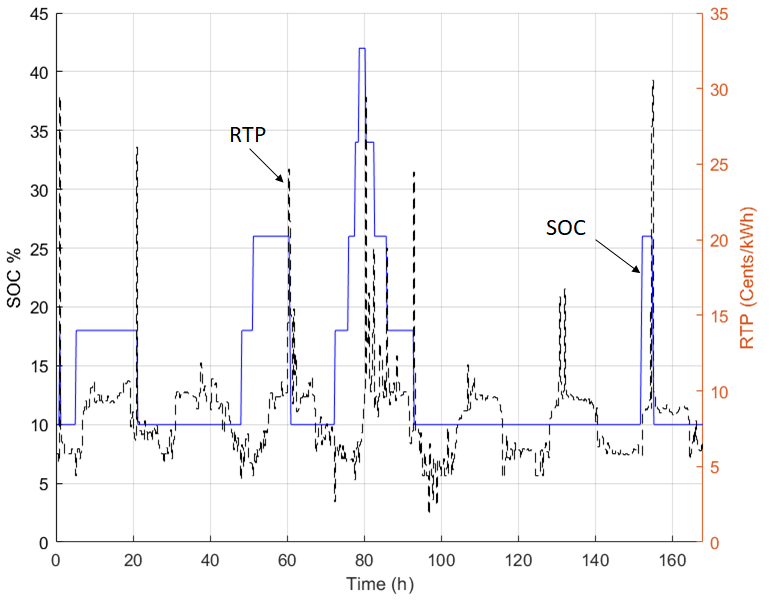
\includegraphics[width = 0.8\linewidth]{figs/SBMPO_COMP_10_12.png}
    \caption{Full 7 day EMS response for net metering comparison case}
    \label{fig:SBMPO_COMP_10_12}
\end{figure}

\subsection{Scenario II: Buying and selling prices are different}
In this scenario, the proposed algorithm is tested against the two base test cases using different price for selling power back to the grid. The cases 1 and 2 are previously fixed standard control strategies based on predefined charging and discharging of the energy storage mentioned before. The only difference is that the buying and selling price of energy from the grid is not the RTP. It is considered that the consumer is only allowed to sell power back to the grid at a rate of 4 cents/kWh.

Fig. \ref{fig:VAR_1_day_example} shows the 1-day test result for the A*-based EMS considering the RTP scheme shown in Fig. \ref{fig:RTP_PROFILE_8} for buying power and considering a sell-back price of 4 cents/kWh. The other system parameters are kept the same as the system used in the previous scenario. As seen in Fig. \ref{fig:VAR_1_day_example}, there are two peaks in price at points 1 and 3 throughout the 24-hour window of operation. The ESM properly anticipates the peak at point 1 and charges the energy storage using the grid just before the peak occurs and discharges during the price peak at point 1, similar to the behavior observed in the previous scenario. The next price peak is at point 3, and the lowest price for grid power available for charging the storage is at point 4. In case of a net metering scheme, point 4 would have been the best time to charge the ES in order to discharge it during the next price peak. However, because a sell-back price of 4 cents/kWh is being considered, this is no longer the case. The price 4 cents/kWh is lower than the price of buying grid energy at point 4. So the A*-based EMS takes into account that the opportunity cost for using power during point 2 instead of selling it back to the grid is 4 cents/kWh and decides to charge the ES during point 2 when there is additional local generation available. This behavior demonstrates that the A*-based ESM can use the forecasted knowledge of the future demand and RTP together to automatically decide the best moments to operate the energy storage depending on different pricing schemes.

 \begin{figure}[!ht]
    \centering
    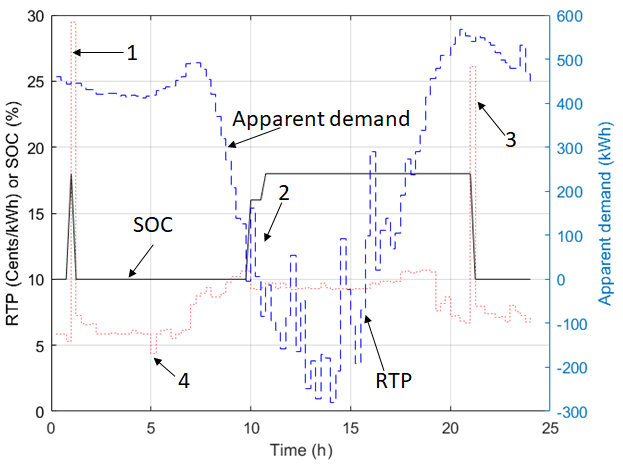
\includegraphics[width = 0.8\linewidth]{figs/VAR_1_day_example.png}
    \caption{1 day EMS response considering NYISO price and 4 centes/kWh sellback price}
    \label{fig:VAR_1_day_example}
\end{figure}

Fig. \ref{fig:VAR_10_12_4} shows the 7-day test result for the tested microgrid considering the RTP shown in Fig. \ref{fig:RTP_PROFILE_8} and a sell-back price of 4 cents/kWh. Fig. \ref{fig:PG_VAR_10_12_4} show the ESM operation for the PG\&E profile shown in Fig. \ref{fig:RTP_PROFILE_8} considering 4 cents/kWh sell-back price. It can be observed from the 7-day cases, that the A*-based ESM shows behavior similar to the behavior seen in  Fig. \ref{fig:VAR_1_day_example}. The ESM scheme was also tested considering a sell-back price of 30\% of RTP for both the NYISO and PG\&E price profiles. The costs for the different conditions considered in the three cases are shown in Table \ref{tab:Cost}. Depending on the test case evaluated, the A* based ESM shows substantial cost savings of around 6.93\% to 41.79\%. 

 \begin{figure}[!ht]
    \centering
    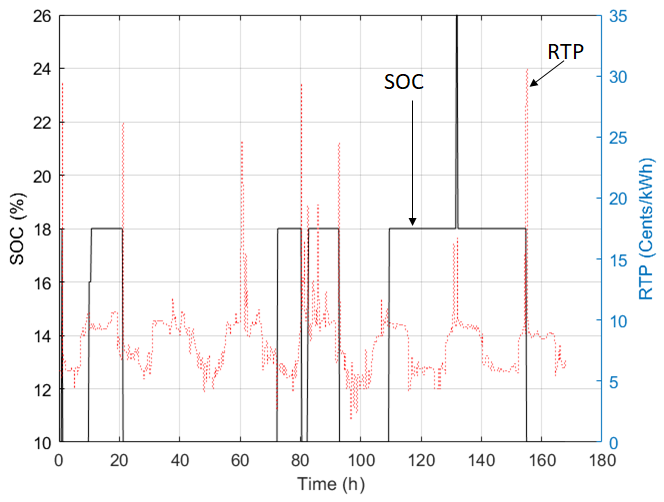
\includegraphics[width = 0.8\linewidth]{figs/VAR_10_12_4.png}
    \caption{7 day EMS response considering NYISO price and 4 centes/kWh sell back price}
    \label{fig:VAR_10_12_4}
\end{figure}

%  \begin{figure}[!ht]
%     \centering
%     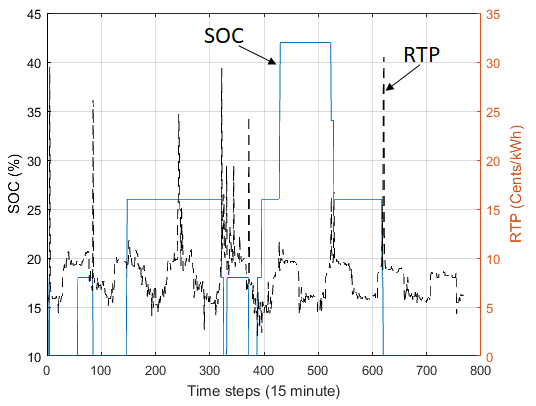
\includegraphics[width = \linewidth]{figs/VAR_10_12_30rtp.png}
%     \caption{7 day EMS response considering NYISO price and 30\% of RTP sell back price}
%     \label{fig:VAR_10_12_30rtp}
% \end{figure}

 \begin{figure}[!ht]
    \centering
    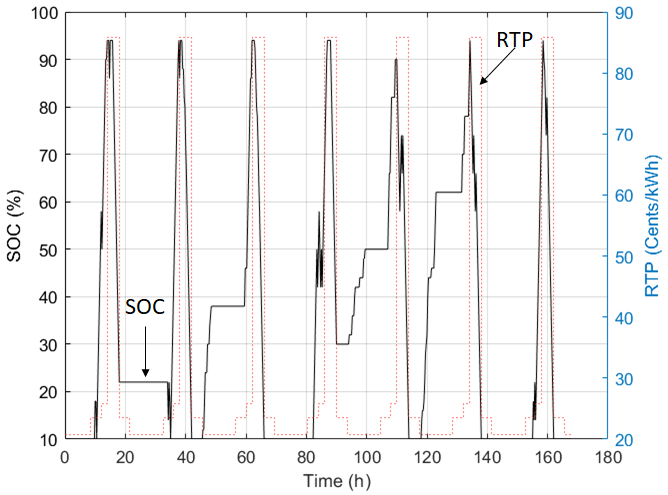
\includegraphics[width = 0.8\linewidth]{figs/PG_VAR_10_12_4.png}
    \caption{7 day EMS response considering PG\&E price and 4 centes/kWh sell back price}
    \label{fig:PG_VAR_10_12_4}
\end{figure}

%  \begin{figure}[!ht]
%     \centering
%     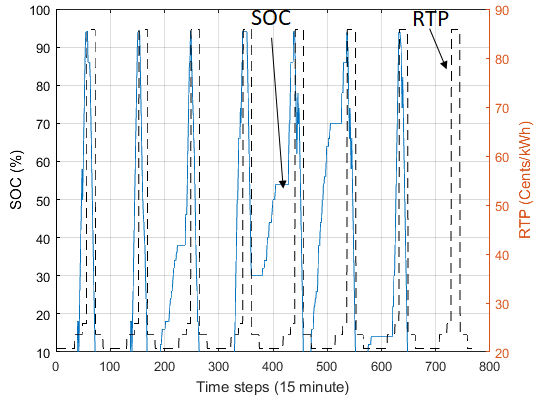
\includegraphics[width = \linewidth]{figs/PG_VAR_10_12_30rtp.png}
%     \caption{7 day EMS response considering PG\&E price and 30\% of RTP sell back price}
%     \label{fig:PG_VAR_10_12_30rtp}
% \end{figure}


%%%%%%%%CSOT%%%%%%%%%%%%%%%%%%%%%%%%%%%%%%%%%%%
\begin{table}[htb]
%\normalsize
%\renewcommand{\arraystretch}{1}
\caption{Seven day Cost for different sell price cases}
\label{tab:Cost}
\centering

\begin{tabular}{l|l|l|l|l|}
\cline{2-5}
                            & \multicolumn{2}{l|}{4 cents/kWh} & \multicolumn{2}{l|}{30\% RTP}   \\ \cline{2-5} 
                            & NYISO           & PG\&E          & NYISO          & PG\&E          \\ \hline
\multicolumn{1}{|l|}{Case1 cost} & \$8,265  & \$19,396 & \$8,314 & \$19,109 \\ \hline
\multicolumn{1}{|l|}{Case2 cost} & \$8,860  & \$19,633 & \$8,895 & \$19,407 \\ \hline
\multicolumn{1}{|l|}{A* Case cost} & \$5,329  & \$18,051 & \$5,178 & \$17,106 \\ \hline
\multicolumn{1}{|l|}{A* Case \% savings (Case1)} & 35.52\%         & 6.93\%         & 37.72\%        & 10.84\%        \\ \hline
\multicolumn{1}{|l|}{A* Case \% savings (Case2)} & 39.85\%         & 8.08\%         & 41.79\%        & 11.86\%        \\ \hline
\end{tabular}

\end{table}
%%%%%%%%CSOT%%%%%%%%%%%%%%%%%%%%%%%%%%%%%%%%%%%%%%%%%%%

%%%%%%%%COMPARE_COST%%%%%%%%%%%%%%%%%%%%%%%%%%%%%%%%%%%
% \begin{table}[htb]
% %\normalsize
% %\renewcommand{\arraystretch}{1}
% \caption{Case 3 savings compared to other cases (7 days)}
% \label{tab:Cost_comp}
% \centering
% \begin{tabular}{l|l|l|l|l|}
% \cline{2-5}
%                             & \multicolumn{2}{l|}{4 cents/kWh} & \multicolumn{2}{l|}{30\% RTP}   \\ \cline{2-5} 
%                             & NYISO           & PG\&E          & NYISO          & PG\&E          \\ \hline
% \multicolumn{1}{|l|}{Case1} & 35.52\%         & 6.93\%         & 37.72\%        & 10.84\%        \\ \hline
% \multicolumn{1}{|l|}{Case2} & 39.85\%         & 8.08\%         & 41.79\%        & 11.86\%        \\ \hline
% \end{tabular}
% \end{table}
% %%%%%%%%COMPARE_COST%%%%%%%%%%%%%%%%%%%%%%%%%%%%%%%%%%%